\documentclass[aps,nofootinbib,notitlepage,11pt]{revtex4-1}

% linking references
\usepackage{hyperref}
\hypersetup{
  breaklinks=true,
  colorlinks=true,
  linkcolor=blue,
  filecolor=magenta,
  urlcolor=cyan,
}

%%% symbols, notations, etc.
\usepackage{physics,braket,bm,amssymb} % physics and math
\renewcommand{\t}{\text} % text in math mode
\newcommand{\f}[2]{\dfrac{#1}{#2}} % shorthand for fractions
\newcommand{\p}[1]{\left(#1\right)} % parenthesis
\renewcommand{\sp}[1]{\left[#1\right]} % square parenthesis
\renewcommand{\set}[1]{\left\{#1\right\}} % curly parenthesis
\renewcommand{\v}{\bm} % bold vectors
\newcommand{\uv}[1]{\hat{\v{#1}}} % unit vectors
\newcommand{\av}{\vec} % arrow vectors
\newcommand{\del}{\nabla} % del operator
\renewcommand{\d}{\partial} % partial d
\renewcommand{\c}{\cdot} % inner product
\newcommand{\w}{\wedge} % wedge product
\newcommand{\bk}{\Braket} % shorthand for braket notation

\newcommand{\up}{\uparrow}
\newcommand{\dn}{\downarrow}
\newcommand{\g}{\text{g}}
\newcommand{\e}{\text{e}}
\renewcommand{\L}{\text{L}}
\newcommand{\C}{\text{C}}
\newcommand{\R}{\text{R}}
\newcommand{\B}{\text{B}}
\renewcommand{\P}{\text{P}}
\newcommand{\T}{\text{T}}

\usepackage{dsfont} % for \1
\newcommand{\1}{\mathds{1}}

\usepackage{mathtools} % for coloneqq
\usepackage{tikz} % for energy level diagram
\tikzset{
  baseline = (current bounding box.center),
}
\usetikzlibrary{decorations.pathmorphing}


\usepackage[inline]{enumitem} % in-line lists

% leave a note in the text, visible in the compiled document
\newcommand{\note}[1]{\textcolor{red}{#1}}

\begin{document}

\title{Basic operations for a quantum link model with ultracold
  $^{87}$Sr on a lattice}

\author{Michael A. Perlin}

\maketitle

We consider loading ultracold $^{87}$Sr atoms into an isolated
three-site cell of a state-dependent 2-D optical superlattice, with
real on-sites wavefunctions $\phi_\L$ (left) and $\phi_\R$ (right) for
atoms in the ground electronic state ($^1S_0$), and $\phi_\C$ (center)
for atoms in the excited electronic state ($^3P_0$).  The
single-particle Hamiltonian is then
\begin{align}
  H_0 = \sum_{s,\mu} E_s c_{s\mu}^\dag c_{s\mu},
\end{align}
for sites $r,s\in\set{\L,\C,\R}$, nuclear spins
$\mu\in\set{-I,\cdots,I}$, and fermionic annihilation operators
$c_{s\mu}$.  The energy mismatches $\Delta_{pq}\equiv E_p-E_q$ between
sites $p\ne q$ will generally set the largest energy scale throughout
this work.  If there are multiple atoms loaded within the same cell,
these atoms interact through the two-body Hamiltonian
\begin{align}
  H_{\t{int}} = \f12 \sum_{\substack{p,q,r,s\\\mu,\nu}}
  V^{pq}_{rs} c_{r\mu}^\dag c_{s\nu}^\dag c_{q\nu} c_{p\mu}
  \label{eq:H_int_full}
\end{align}
for interaction strengths $V^{pq}_{rs}$ which depend only on the sites
and their associated electronic states; these interaction strengths do
not depend on the nuclear spin states involved.  Defining
\begin{align}
  K^{pq}_{rs} \equiv \int d^3x~ \phi_r^* \phi_s^* \phi_q \phi_p,
  &&
  G_{\sigma=\g,\e} \equiv \f{4\pi}{m_A} a_{\sigma\sigma},
  &&
  G_\pm \equiv \f{2\pi}{m_A} \p{a_{\e\g+} \pm a_{\e\g-}},
\end{align}
\begin{align}
  G^{\alpha\beta}_{\gamma\delta} \equiv \left\{
    \begin{array}{ll}
      G_\alpha & ~ \alpha = \beta = \gamma = \delta \\
      G_+ & ~ \alpha \ne \beta ~ \t{and} ~
            (\alpha,\beta) = (\gamma,\delta) \\
      G_- & ~ \alpha \ne \beta ~ \t{and} ~
            (\alpha,\beta) = (\delta,\gamma) \\
      0 & ~ \t{otherwise}
    \end{array}\right.,
\end{align}
for an atomic mass $m_A$ and scattering lengths $a_X$, the interaction
strengths in \eqref{eq:H_int_full} are
\begin{align}
  V^{pq}_{rs} = K^{pq}_{rs}
  G^{\varepsilon\p{p}\varepsilon\p{q}}_{\varepsilon\p{r}\varepsilon\p{s}},
\end{align}
where $\varepsilon\p{p}\in\set{\g,\e}$ selects the electronic state
associated with site $p$.  As a first approximation, we assume that
the two-body overlap integral $K^{pq}_{rs}$ is negligible unless
$\set{p,q}=\set{r,s}$, i.e. we neglect interaction-assisted tunneling
in $H_{\t{int}}$.  In the presence of only $H_0$ and $H_{\t{int}}$,
this approximation can also be justified by the secular approximation
due to mismatched single-particle on-site energies $E_s$.  The
interaction Hamiltonian then simplifies to
\begin{align}
  H_{\t{int}}
  = \f12 \sum_{p,\mu,\nu} V_p c_{p\mu}^\dag c_{p\nu}^\dag c_{p\nu} c_{p\mu}
  + \f12 \sum_{\substack{p\ne q\\\mu,\nu}} V_{pq}
  \p{c_{p\mu}^\dag c_{q\nu}^\dag c_{q\nu} c_{p\mu}
    + c_{q\mu}^\dag c_{p\nu}^\dag c_{q\nu} c_{p\mu}},
  \label{eq:H_int_two}
\end{align}
where
\begin{align}
  V_p \equiv V^{pp}_{pp},
  &&
  V_{pq} \equiv V^{pq}_{pq} = V^{pq}_{qp},
  &&
  n_{p\mu} \equiv c_{p\mu}^\dag c_{p\mu}.
\end{align}
As made clear by the form in \eqref{eq:H_int_two}, the interaction
Hamiltonian $H_{\t{int}}$ generally induces nuclear spin exchange
between atoms in different orbitals.  In order to suppress nuclear
spin exchange, we further restrict ourselves to a regime in which the
two-body overlap integral $K^{pq}_{rs}$ is negligible unless all atoms
are on the same site (i.e. unless $p=q=r=s$), such that
\begin{align}
  H_{\t{int}}
  = \f12 \sum_{p,\mu,\nu} V_p c_{p\mu}^\dag c_{p\nu}^\dag c_{p\nu} c_{p\mu}
  = \sum_{\substack{p\\\mu<\nu}} V_p n_{p\mu} n_{p\nu}.
  \label{eq:H_int}
\end{align}
Throughout the remainder of this work, to simplify matters we
generally assume that atoms initially in the electronic ground state
on site $\L$ or $\R$ lie in the nuclear spin manifold spanned by
$\set{\ket{-I},\ket{-I+1}}$, while atoms initially in an excited
electronic state on site $\C$ lie in the nuclear spin manifold spanned
by $\set{\ket{I},\ket{I-1}}$.  We also assume that each site is
initially populated with at most one atom.


\section{Global control gates}
\label{sec:global_control}

We wish to build a toolkit of operations to manipulate atoms in our
three-site cell, with the long term goal of combining many such cells
to simulate a quantum link model.  Before we discuss any multi-body
gates, we first need to construct some basic, single-body global
control operations.  These basic operations together with the two-body
interaction Hamiltonian $H_{\t{int}}$ in \eqref{eq:H_int} will be our
building blocks for realizing more complicated gates.

The first simple operation we consider is the application of a static
magnetic field with strength $B$ along the nuclear spin quantization
axis (which we will generally keep fixed), realizing the Hamiltonian
\begin{align}
  H_\B = -\gamma_{\text{n}} B \sum_{s,\mu} \mu n_{s\mu},
\end{align}
where $\gamma_{\text{n}}$ is the nuclear gyromagnetic ratio.  Applying
this Hamiltonian for a time $t=\theta/\gamma_nB$ generates the phase
gate
\begin{align}
  U_\B\p{\theta} = \sum_{s,\mu} e^{i \theta \mu} n_{s\mu}.
\end{align}
As the nuclear spins $\mu$ are half-integers, the operation
$U_\B\p{\theta}$ is periodic in $\theta$ with period $4\pi$.

We can also shine an auxiliary laser with angular frequency $\omega$
to apply the Hamiltonian
\begin{align}
  H_\Omega^{(\sigma)}
  = - \sum_\mu e^{i\omega t}
  \p{\Omega_{\C,\L,\mu}^{(\sigma)} c_{\L,\mu}^\dag
    + \Omega_{\C,\R,\mu}^{(\sigma)} c_{\R,\mu}^\dag} c_{\C,\mu+\sigma}
  + \t{h.c.},
\end{align}
where $\sigma\in\set{-1,0,1}$ is determined by the clock laser
polarization; $\L\leftrightarrow\R$ coupling is forbidden because
$H_\Omega^{(\sigma)}$ is strictly off-diagonal in electronic state;
and $\t{h.c.}$ denotes the Hermitian conjugate, i.e.
$X+\t{h.c.}\equiv X+X^\dag$.  By evaluating the Clebsch-Gordan
coefficients $\bk{I,\mu+\sigma;1,-\sigma|I,\mu}$, we can extract the
$\mu,\sigma,p,q$ dependence of $\Omega_{pq\mu}^{(\sigma)}$ to find
\begin{align}
  \Omega_{pq\mu}^{(0)} = \Omega_{pq}^{(0)} \mu,
  &&
  \Omega_{pq\mu}^{(\pm1)} = \pm \Omega_{pq}^{(1)}
  \sqrt{\p{I\mp\mu}\p{I\pm\mu+1}},
  &&
  \Omega_{pq}^{(\sigma)} \equiv \Omega_\sigma \int d^3x~ \phi_q^* \phi_p,
\end{align}
for experimentally tunable intensities $\Omega_0$ and $\Omega_1$ which
are independent of nuclear spin and lattice site.  In this section, we
will generally assume that these intensities are real and large
compared to all interaction energies,
i.e. $\Omega_0,\Omega_1\gg\max_p\abs{V_p}$.  We also consider the case
of ${}^{87}$Sr with net nuclear spin $I=9/2$ in order to fix the
relative magnitudes of couplings $\Omega_{pq\mu}^{(\sigma)}$ for
different nuclear spins $\mu$.  The Hamiltonians $H_\Omega^{(\sigma)}$
can be thought of diagrammatically as
\begin{align}
  H_\Omega^{(0)} \sim
  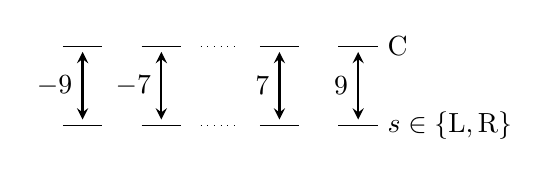
\begin{tikzpicture}[
    scale=0.5,
    trans/.style={thick,<->,shorten >=2pt,shorten <=2pt,>=stealth}
    ]
    \draw (0,0) -- (1,0);
    \draw (2,0) -- (3,0);
    \draw[dotted] (3.5,0) -- (4.5,0);
    \draw (5,0) -- (6,0);
    \draw (7,0) -- (8,0);
    \draw (7,0) -- (8,0) node[right] {$\C$};
    \draw (0,-2) -- (1,-2);
    \draw (2,-2) -- (3,-2);
    \draw[dotted] (3.5,-2) -- (4.5,-2);
    \draw (5,-2) -- (6,-2);
    \draw (7,-2) -- (8,-2);
    \draw (7,-2) -- (8,-2) node[right] {$s\in\set{\L,\R}$};
    \draw[trans] (0.5,0) -- (0.5,-2) node[midway,left] {$-9$};
    \draw[trans] (2.5,0) -- (2.5,-2) node[midway,left] {$-7$};
    \draw[trans] (5.5,0) -- (5.5,-2) node[midway,left] {$7$};
    \draw[trans] (7.5,0) -- (7.5,-2) node[midway,left] {$9$};
  \end{tikzpicture},
\end{align}
where the horizontal lines represent nuclear spin levels from $-9/2$
to $9/2$ (i.e. from left to right) within each orbital state $\C$ or
$s\in\set{\L,\R}$, and the double-headed arrows represent a coupling
between two states.  The numbers next to the arrows represents the
relative magnitudes of the couplings.  Similarly,
\begin{align}
  H_\Omega^{(1)} \sim
  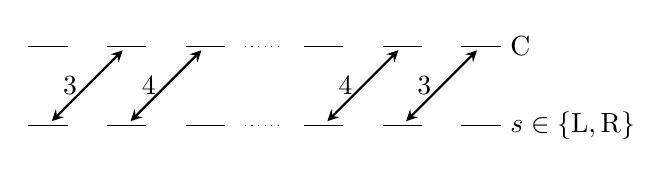
\begin{tikzpicture}[
    scale=0.5,
    trans/.style={thick,<->,shorten >=2pt,shorten <=2pt,>=stealth}
    ]
    \draw (0,0) -- (1,0);
    \draw (2,0) -- (3,0);
    \draw (4,0) -- (5,0);
    \draw[dotted] (5.5,0) -- (6.5,0);
    \draw (7,0) -- (8,0);
    \draw (9,0) -- (10,0);
    \draw (11,0) -- (12,0);
    \draw (11,0) -- (12,0) node[right] {$\C$};
    \draw (0,-2) -- (1,-2);
    \draw (2,-2) -- (3,-2);
    \draw (4,-2) -- (5,-2);
    \draw[dotted] (5.5,-2) -- (6.5,-2);
    \draw (7,-2) -- (8,-2);
    \draw (9,-2) -- (10,-2);
    \draw (11,-2) -- (12,-2);
    \draw (11,-2) -- (12,-2) node[right] {$s\in\set{\L,\R}$};
    \draw[trans] (0.5,-2) -- (2.5,0) node[midway,left] {$3$};
    \draw[trans] (2.5,-2) -- (4.5,0) node[midway,left] {$4$};
    \draw[trans] (7.5,-2) -- (9.5,0) node[midway,left] {$4$};
    \draw[trans] (9.5,-2) -- (11.5,0) node[midway,left] {$3$};
  \end{tikzpicture},
  \label{eq:H_O_+}
\end{align}
and
\begin{align}
  H_\Omega^{(-1)} \sim
  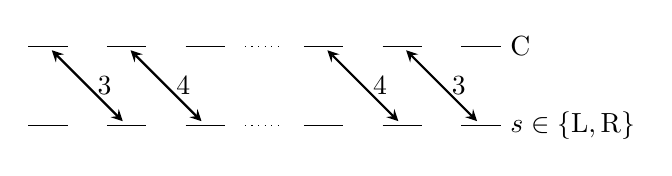
\begin{tikzpicture}[
    scale=0.5,
    trans/.style={thick,<->,shorten >=2pt,shorten <=2pt,>=stealth}
    ]
    \draw (0,0) -- (1,0);
    \draw (2,0) -- (3,0);
    \draw (4,0) -- (5,0);
    \draw[dotted] (5.5,0) -- (6.5,0);
    \draw (7,0) -- (8,0);
    \draw (9,0) -- (10,0);
    \draw (11,0) -- (12,0);
    \draw (11,0) -- (12,0) node[right] {$\C$};
    \draw (0,-2) -- (1,-2);
    \draw (2,-2) -- (3,-2);
    \draw (4,-2) -- (5,-2);
    \draw[dotted] (5.5,-2) -- (6.5,-2);
    \draw (7,-2) -- (8,-2);
    \draw (9,-2) -- (10,-2);
    \draw (11,-2) -- (12,-2);
    \draw (11,-2) -- (12,-2) node[right] {$s\in\set{\L,\R}$};
    \draw[trans] (0.5,0) -- (2.5,-2) node[midway,right] {$3$};
    \draw[trans] (2.5,0) -- (4.5,-2) node[midway,right] {$4$};
    \draw[trans] (7.5,0) -- (9.5,-2) node[midway,right] {$4$};
    \draw[trans] (9.5,0) -- (11.5,-2) node[midway,right] {$3$};
  \end{tikzpicture},
  \label{eq:H_O_-}
\end{align}
where we neglect couplings for nuclear spins $\mu$ outside of
$\set{-I,-I+1,I-1,I}$.

By turning on $H_\Omega^{(0)}$ for a time $t=\pi/\Omega^{(0)}_{\C,s}$
with an angular frequency $\omega$ resonant on the energy difference
$\Delta_{\C,s}=E_C-E_s$ for $s\in\set{\L,\R}$, we can apply the
$\pi$-pulse gate
\begin{align}
  U_{\pi,s}
  \equiv \sum_\mu e^{i\pi\mu} c_{s\mu}^\dag c_{\C,\mu} + \t{h.c}
  \coloneqq i \times
  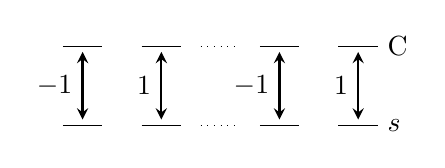
\begin{tikzpicture}[
    scale=0.5,
    trans/.style={thick,<->,shorten >=2pt,shorten <=2pt,>=stealth}
    ]
    \draw (0,0) -- (1,0);
    \draw (2,0) -- (3,0);
    \draw[dotted] (3.5,0) -- (4.5,0);
    \draw (5,0) -- (6,0);
    \draw (7,0) -- (8,0);
    \draw (7,0) -- (8,0) node[right] {$\C$};
    \draw (0,-2) -- (1,-2);
    \draw (2,-2) -- (3,-2);
    \draw[dotted] (3.5,-2) -- (4.5,-2);
    \draw (5,-2) -- (6,-2);
    \draw (7,-2) -- (8,-2);
    \draw (7,-2) -- (8,-2) node[right] {$s$};
    \draw[trans] (0.5,0) -- (0.5,-2) node[midway,left] {$-1$};
    \draw[trans] (2.5,0) -- (2.5,-2) node[midway,left] {$1$};
    \draw[trans] (5.5,0) -- (5.5,-2) node[midway,left] {$-1$};
    \draw[trans] (7.5,0) -- (7.5,-2) node[midway,left] {$1$};
  \end{tikzpicture},
  \label{eq:U_pi}
\end{align}
which swaps atoms between orbitals $\C$ and $s$ and applies a
spin-dependent sign.

The relative magnitudes of the couplings $\Omega_{pq\mu}^{(\pm1)}$ for
different nuclear spins $\mu$ similarly allows us to turn on
$H_\Omega^{(\pm1)}$ for an appropriately resonant angular frequency
$\omega$ and a time $t=\p{\pi/2}/\Omega_{\C,s}^{(1)}$, thereby
realizing the gates
\begin{align}
  U_{\pi,s}^+
  \equiv -i\p{c_{s,-I+1} c_{\C,-I+1}^\dag + c_{s,I-1}^\dag c_{\C,I}}
  + \t{h.c.}
  \coloneqq -i \times
  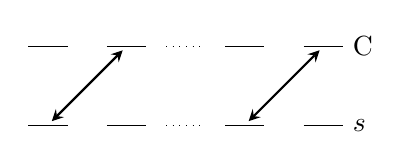
\begin{tikzpicture}[
    scale=0.5,
    trans/.style={thick,<->,shorten >=2pt,shorten <=2pt,>=stealth}
    ]
    \draw (0,0) -- (1,0);
    \draw (2,0) -- (3,0);
    \draw[dotted] (3.5,0) -- (4.5,0);
    \draw (5,0) -- (6,0);
    \draw (7,0) -- (8,0);
    \draw (7,0) -- (8,0) node[right] {$\C$};
    \draw (0,-2) -- (1,-2);
    \draw (2,-2) -- (3,-2);
    \draw[dotted] (3.5,-2) -- (4.5,-2);
    \draw (5,-2) -- (6,-2);
    \draw (7,-2) -- (8,-2);
    \draw (7,-2) -- (8,-2) node[right] {$s$};
    \draw[trans] (2.5,0) -- (0.5,-2);
    \draw[trans] (7.5,0) -- (5.5,-2);
  \end{tikzpicture},
  \label{eq:U_pi_+}
\end{align}
and
\begin{align}
  U_{\pi,s}^-
  \equiv i\p{c_{s,-I+1} c_{\C,-I+1}^\dag + c_{s,I}^\dag c_{\C,I-1}}
  + \t{h.c.}
  \coloneqq i \times
  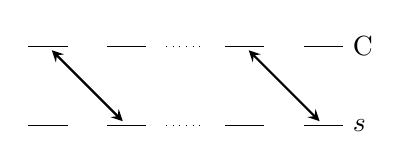
\begin{tikzpicture}[
    scale=0.5,
    trans/.style={thick,<->,shorten >=2pt,shorten <=2pt,>=stealth}
    ]
    \draw (0,0) -- (1,0);
    \draw (2,0) -- (3,0);
    \draw[dotted] (3.5,0) -- (4.5,0);
    \draw (5,0) -- (6,0);
    \draw (7,0) -- (8,0);
    \draw (7,0) -- (8,0) node[right] {$\C$};
    \draw (0,-2) -- (1,-2);
    \draw (2,-2) -- (3,-2);
    \draw[dotted] (3.5,-2) -- (4.5,-2);
    \draw (5,-2) -- (6,-2);
    \draw (7,-2) -- (8,-2);
    \draw (7,-2) -- (8,-2) node[right] {$s$};
    \draw[trans] (0.5,0) -- (2.5,-2);
    \draw[trans] (5.5,0) -- (7.5,-2);
  \end{tikzpicture},
  \label{eq:U_pi_-}
\end{align}
where the remaining states addressed by $H_\Omega^{(\pm1)}$ in
\eqref{eq:H_O_+} and \eqref{eq:H_O_-} are unaffected because they
undergo Rabi cycles which bring them back to their initial states.

All of the above $\pi$-pulse gates can be turned into $\pi/2$-pulse
gates $U_{\pi/2,s}$, $U_{\pi/2,s}^\pm$ simply by applying the
appropriate Hamiltonian for half of the specified time.  Furthermore,
if we are guaranteed that only certain nuclear spin states are
occupied, we can also apply $\pi$-pulse gates by turning on
$H_\Omega^{(\pm1)}$ for a time $t=\p{\pi/6}/\Omega_{\C,s}^{(1)}$,
giving us
\begin{align}
  \tilde U_{\pi,s}^+
  \coloneqq i \times
  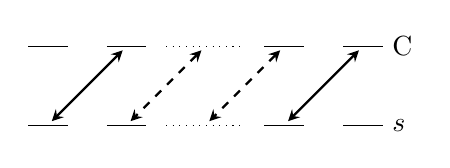
\begin{tikzpicture}[
    scale=0.5,
    trans/.style={thick,<->,shorten >=2pt,shorten <=2pt,>=stealth}
    ]
    \draw (0,0) -- (1,0);
    \draw (2,0) -- (3,0);
    \draw[dotted] (3.5,0) -- (5.5,0);
    \draw (6,0) -- (7,0);
    \draw (8,0) -- (9,0);
    \draw (8,0) -- (9,0) node[right] {$\C$};
    \draw (0,-2) -- (1,-2);
    \draw (2,-2) -- (3,-2);
    \draw[dotted] (3.5,-2) -- (5.5,-2);
    \draw (6,-2) -- (7,-2);
    \draw (8,-2) -- (9,-2);
    \draw (8,-2) -- (9,-2) node[right] {$s$};
    \draw[trans] (2.5,0) -- (0.5,-2);
    \draw[trans, dashed] (4.5,0) -- (2.5,-2);
    \draw[trans, dashed] (6.5,0) -- (4.5,-2);
    \draw[trans] (8.5,0) -- (6.5,-2);
  \end{tikzpicture},
  &&
  \tilde U_{\pi,s}^-
  \coloneqq -i \times
  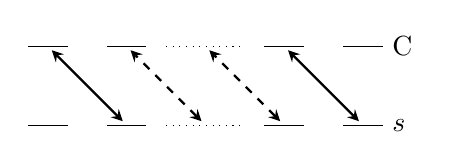
\begin{tikzpicture}[
    scale=0.5,
    trans/.style={thick,<->,shorten >=2pt,shorten <=2pt,>=stealth}
    ]
    \draw (0,0) -- (1,0);
    \draw (2,0) -- (3,0);
    \draw[dotted] (3.5,0) -- (5.5,0);
    \draw (6,0) -- (7,0);
    \draw (8,0) -- (9,0);
    \draw (8,0) -- (9,0) node[right] {$\C$};
    \draw (0,-2) -- (1,-2);
    \draw (2,-2) -- (3,-2);
    \draw[dotted] (3.5,-2) -- (5.5,-2);
    \draw (6,-2) -- (7,-2);
    \draw (8,-2) -- (9,-2);
    \draw (8,-2) -- (9,-2) node[right] {$s$};
    \draw[trans] (2.5,-2) -- (0.5,0);
    \draw[trans, dashed] (4.5,-2) -- (2.5,0);
    \draw[trans, dashed] (6.5,-2) -- (4.5,0);
    \draw[trans] (8.5,-2) -- (6.5,0);
  \end{tikzpicture},
\end{align}
where the dashed arrows indicate incomplete Rabi cycles that mix nuclear
spin states in our target subspace with those outside it.  For
simplicity, we will work strictly with the cleaner $\pi$-pulse gates
in \eqref{eq:U_pi}, \eqref{eq:U_pi_+}, and \eqref{eq:U_pi_-}.


\section{Tunneling gates}
\label{sec:tunneling}

In order to suppress nuclear spin exchange processes, we restricted
ourselves to a regime in which two-body overlap integrals for pairs of
atoms on different sites vanish.  The on-site wavefunctions $\phi_p$
are therefore fairly localized to site $p$, with some overlap in the
support of $\phi_\C$ with $\phi_s$ for $s\in\set{\L,\R}$ to allow for
the control gates $U_{\pi,s}^\pm$.  As a consequence, we expect
vanishing mutual support of $\phi_\L$ and $\phi_\R$, which means that
we cannot induce $\L\leftrightarrow\R$ tunneling directly.
Nonetheless, we can use the $\pi$-pulse gates $U_{\pi,s}$ in
\eqref{eq:U_pi} to induce indirect $\L\leftrightarrow\R$ tunneling
through the central site $\C$ via
\begin{multline}
  U_\pi^\T
  \equiv U_{\pi,\L} U_{\pi,\R} U_{\pi,\L}
  \cong U_{\pi,\R} U_{\pi,\L} U_{\pi,\R} \\
  \cong
  \sp{\begin{tikzpicture}[
      scale=0.5,
      trans/.style={thick,<->,shorten >=2pt,shorten <=2pt,>=stealth}
      ]
      \draw (0,0) -- (1,0);
      \draw (2,0) -- (3,0);
      \draw[dotted] (3.5,0) -- (4.5,0);
      \draw (5,0) -- (6,0);
      \draw (7,0) -- (8,0);
      \draw (7,0) -- (8,0) node[right] {$\L$};
      \draw (0,-2) -- (1,-2);
      \draw (2,-2) -- (3,-2);
      \draw[dotted] (3.5,-2) -- (4.5,-2);
      \draw (5,-2) -- (6,-2);
      \draw (7,-2) -- (8,-2);
      \draw (7,-2) -- (8,-2) node[right] {$\C$};
      \draw (0,-4) -- (1,-4);
      \draw (2,-4) -- (3,-4);
      \draw[dotted] (3.5,-4) -- (4.5,-4);
      \draw (5,-4) -- (6,-4);
      \draw (7,-4) -- (8,-4);
      \draw (7,-4) -- (8,-4) node[right] {$\R$};
      \draw[trans] (0.5,0) -- (0.5,-2);
      \draw[trans] (2.5,0) -- (2.5,-2);
      \draw[trans] (5.5,0) -- (5.5,-2);
      \draw[trans] (7.5,0) -- (7.5,-2);
    \end{tikzpicture}}
  \sp{\begin{tikzpicture}[
      scale=0.5,
      trans/.style={thick,<->,shorten >=2pt,shorten <=2pt,>=stealth}
      ]
      \draw (0,0) -- (1,0);
      \draw (2,0) -- (3,0);
      \draw[dotted] (3.5,0) -- (4.5,0);
      \draw (5,0) -- (6,0);
      \draw (7,0) -- (8,0);
      \draw (7,0) -- (8,0) node[right] {$\L$};
      \draw (0,-2) -- (1,-2);
      \draw (2,-2) -- (3,-2);
      \draw[dotted] (3.5,-2) -- (4.5,-2);
      \draw (5,-2) -- (6,-2);
      \draw (7,-2) -- (8,-2);
      \draw (7,-2) -- (8,-2) node[right] {$\C$};
      \draw (0,-4) -- (1,-4);
      \draw (2,-4) -- (3,-4);
      \draw[dotted] (3.5,-4) -- (4.5,-4);
      \draw (5,-4) -- (6,-4);
      \draw (7,-4) -- (8,-4);
      \draw (7,-4) -- (8,-4) node[right] {$\R$};
      \draw[trans] (0.5,-2) -- (0.5,-4);
      \draw[trans] (2.5,-2) -- (2.5,-4);
      \draw[trans] (5.5,-2) -- (5.5,-4);
      \draw[trans] (7.5,-2) -- (7.5,-4);
    \end{tikzpicture}}
  \sp{\begin{tikzpicture}[
      scale=0.5,
      trans/.style={thick,<->,shorten >=2pt,shorten <=2pt,>=stealth}
      ]
      \draw (0,0) -- (1,0);
      \draw (2,0) -- (3,0);
      \draw[dotted] (3.5,0) -- (4.5,0);
      \draw (5,0) -- (6,0);
      \draw (7,0) -- (8,0);
      \draw (7,0) -- (8,0) node[right] {$\L$};
      \draw (0,-2) -- (1,-2);
      \draw (2,-2) -- (3,-2);
      \draw[dotted] (3.5,-2) -- (4.5,-2);
      \draw (5,-2) -- (6,-2);
      \draw (7,-2) -- (8,-2);
      \draw (7,-2) -- (8,-2) node[right] {$\C$};
      \draw (0,-4) -- (1,-4);
      \draw (2,-4) -- (3,-4);
      \draw[dotted] (3.5,-4) -- (4.5,-4);
      \draw (5,-4) -- (6,-4);
      \draw (7,-4) -- (8,-4);
      \draw (7,-4) -- (8,-4) node[right] {$\R$};
      \draw[trans] (0.5,0) -- (0.5,-2);
      \draw[trans] (2.5,0) -- (2.5,-2);
      \draw[trans] (5.5,0) -- (5.5,-2);
      \draw[trans] (7.5,0) -- (7.5,-2);
    \end{tikzpicture}} \\
  \cong
  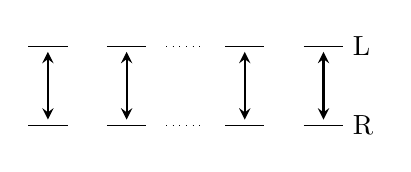
\begin{tikzpicture}[
    scale=0.5,
    trans/.style={thick,<->,shorten >=2pt,shorten <=2pt,>=stealth}
    ]
    \draw (0,0) -- (1,0);
    \draw (2,0) -- (3,0);
    \draw[dotted] (3.5,0) -- (4.5,0);
    \draw (5,0) -- (6,0);
    \draw (7,0) -- (8,0);
    \draw (7,0) -- (8,0) node[right] {$\L$};
    \draw (0,-2) -- (1,-2);
    \draw (2,-2) -- (3,-2);
    \draw[dotted] (3.5,-2) -- (4.5,-2);
    \draw (5,-2) -- (6,-2);
    \draw (7,-2) -- (8,-2);
    \draw (7,-2) -- (8,-2) node[right] {$\R$};
    \draw[trans] (0.5,0) -- (0.5,-2);
    \draw[trans] (2.5,0) -- (2.5,-2);
    \draw[trans] (5.5,0) -- (5.5,-2);
    \draw[trans] (7.5,0) -- (7.5,-2);
  \end{tikzpicture},
  \label{eq:U_pi_T}
\end{multline}
where $\cong$ denotes equality up to an overall phase.  Crucially,
$U_\pi^\T$ swaps atoms between sites $\L$ and $\R$ while leaving atoms
on site $\C$ unaffected.  We can also construct $\pi/2$-pulse gates
for $\L\leftrightarrow\R$ tunneling via
\begin{align}
  U_{\pi/2}^\T
  \equiv U_{\pi,\L} U_{\pi/2,\R} U_{\pi,\L}
  \cong U_{\pi,\R} U_{\pi/2,\L} U_{\pi,\R},
\end{align}
which is identical to the composite gate $U_\pi^\T$ in
\eqref{eq:U_pi_T}, but with a replacement of the second $\pi$-pulse by
a $\pi/2$ pulse.  Finally, we can make use of the
nuclear-spin-selective properties of $U_{\pi,s}^\pm$ to construct
nuclear-spin-selective $\L\leftrightarrow\R$ tunneling gates, simply
by replacing instances of $U_{\pi,s}$ above by $U_{\pi,s}^\pm$.


\section{Controlled-phase gates}
\label{sec:controlled_phase}

We now construct a collisional controlled-phase gate on an atom in
site $\C$, conditional on the presence of an atom in site $s$.  We
first prepare an atom on site $\C$ in the nuclear spin manifold
spanned by $\set{\ket{I},\ket{I-1}}$, and consider the possibility of
an atom on site $s$ with nuclear spin state $\ket{-I}$, preparing the
state
\begin{align}
  \ket{\psi_{sm}}
  = \ket{s,-I;m} \otimes \p{\alpha\ket{\C,I} + \beta\ket{\C,I-1}}
  \sim
  \begin{tikzpicture}[
    scale=0.5,
    sim/.style={decorate, decoration=snake},
    ]
    \draw (0,0) -- (1,0);
    \draw (2,0) -- (3,0);
    \draw[dotted] (3.5,0) -- (4.5,0);
    \draw (5,0) -- (6,0) node[midway, above] {$\beta$};
    \draw (7,0) -- (8,0) node[midway, above] {$\alpha$};
    \draw (7,0) -- (8,0) node[right] {$\C$};
    \draw (0,-2) -- (1,-2) node[midway, above] {$m$};
    \draw (2,-2) -- (3,-2);
    \draw[dotted] (3.5,-2) -- (4.5,-2);
    \draw (5,-2) -- (6,-2);
    \draw (7,-2) -- (8,-2);
    \draw (7,-2) -- (8,-2) node[right] {$s$};
    \draw[sim] (6,0.5) -- (7,0.5);
  \end{tikzpicture}
  \label{eq:psi_sm}
\end{align}
where $m=0$ ($m=1$) marks the absence (presence) of an atom on site
$s$ with spin $-I$.  The above diagram is merely provided as a sketch
of the state; we will make no attempt at making this sketch a formal
representation.

Applying the gate $U_{\pi,s}^-$ in \eqref{eq:U_pi_-} to the state
$\ket{\psi_{sm}}$ in \eqref{eq:psi_sm} gives us
\begin{align}
  U_{\pi,s}^-\ket{\psi_{sm}}
  \cong \ket{s,-I;m} \otimes \p{\alpha\ket{\C,I} + \beta\ket{s,I}}
  \sim
  \begin{tikzpicture}[
    scale=0.5,
    sim/.style={decorate, decoration=snake},
    ]
    \draw (0,0) -- (1,0);
    \draw (2,0) -- (3,0);
    \draw[dotted] (3.5,0) -- (4.5,0);
    \draw (5,0) -- (6,0);
    \draw (7,0) -- (8,0) node[midway, above] {$\alpha$};
    \draw (7,0) -- (8,0) node[right] {$\C$};
    \draw (0,-2) -- (1,-2) node[midway, above] {$m$};
    \draw (2,-2) -- (3,-2);
    \draw[dotted] (3.5,-2) -- (4.5,-2);
    \draw (5,-2) -- (6,-2);
    \draw (7,-2) -- (8,-2) node[midway, above] {$\beta$};
    \draw (7,-2) -- (8,-2) node[right] {$s$};
    \draw[sim] (7.5,0.1) -- (7.5,-0.9);
  \end{tikzpicture}.
\end{align}
Holding for a time $t$ (i.e. evolving under $H_0+H_{\t{int}}$) now
makes $\beta$ pick up a phase relative to $\alpha$ as
$\beta\to\tilde\beta_{sm}\p{t}\equiv\beta e^{it\Delta_{\C,s}-itV_sm}$,
where $\Delta_{\C,s}=E_\C-E_s$ is the single-particle energy
difference between the orbitals $\C$ and $s$, and $V_s$ is the
interaction energy of two atoms in orbital $s$.  Subsequently applying
$U_{\pi,s}^-$ then gives us the state
\begin{align}
  U_{\pi,s}^- U_{\t{hold}}\p{t} U_{\pi,s}^- \ket{\psi_{sm}}
  \cong \ket{s,-I;m} \otimes
  \p{\alpha\ket{\C,I} + \tilde\beta_{sm}\p{t}\ket{\C,I-1}}
  \sim
  \begin{tikzpicture}[
    scale=0.5,
    sim/.style={decorate, decoration=snake},
    ]
    \draw (0,0) -- (1,0);
    \draw (2,0) -- (3,0);
    \draw[dotted] (3.5,0) -- (4.5,0);
    \draw (5,0) -- (6,0) node[near start, above]
    {$\tilde\beta_{sm}\p{t}$};
    \draw (7,0) -- (8,0) node[midway, above] {$\alpha$};
    \draw (7,0) -- (8,0) node[right] {$\C$};
    \draw (0,-2) -- (1,-2) node[midway, above] {$m$};
    \draw (2,-2) -- (3,-2);
    \draw[dotted] (3.5,-2) -- (4.5,-2);
    \draw (5,-2) -- (6,-2);
    \draw (7,-2) -- (8,-2);
    \draw (7,-2) -- (8,-2) node[right] {$s$};
    \draw[sim] (6.5,0.5) -- (7,0.5);
  \end{tikzpicture}.
\end{align}
The extra relative phase $e^{it\Delta_{\C,s}}$ on
$\tilde\beta_{sm}\p{t}$ can be cancelled out by the application of a
magnetic field with $U_\B\p{t\Delta_{\C,s}}$. In the basis
$\ket{m}_s\equiv\ket{s,-I;m}$ for site $s$ and
$\ket{n}_\C\equiv\ket{\C,I-n}$ for site $\C$, the net effect of our
sequence is thus the controlled-phase gate
\begin{multline}
  U_{\P,s}^{(0)}\p{t}
  \equiv U_\B\p{t\Delta_{\C,s}}
  U_{\pi,s}^- U_{\t{hold}}\p{t} U_{\pi,s}^- \\
  = \sum_{m,n\in\set{0,1}} \exp\p{-itV_snm} \op{m}_s\otimes\op{n}_\C
  = \op{0}_s \otimes \1_\C + \op{1}_s \otimes
  \begin{pmatrix}
    1 & 0 \\ 0 & e^{-itV_s}
  \end{pmatrix}_\C.
  \label{eq:U_P_0}
\end{multline}
A similar controlled-phase gate $U_{\P,s}^{(1)}\p{t}$ can be realized
conditional on the presence of an atom on site $s$ with nuclear spin
$-I+1$ by using $U_{\pi,s}^+$ in place of $U_{\pi,s}^-$.  Note that if
the atom on site $s$ is in a nontrivial superposition of nuclear spin
states $\ket{-I}$ and $\ket{-I+1}$, there will be two atoms on site
$\C$ during the hold time of $U_{\P,s}^{(0)}\p{t}$ and
$U_{\P,s}^{(1)}\p{t}$, resulting in atom losses from
${}^3P_0$-${}^3P_0$ interactions.

As a final comment, we mention that if we are guaranteed a single atom
on e.g.  site $\L$ and no atom on site $\R$, we can use the
nuclear-spin selective $\L\leftrightarrow\R$ tunneling gates mentioned
at the end of section \ref{sec:tunneling} to construct a
controlled-phase gate conditional on the nuclear spin of an atom on
site $s$, rather than on the mere presence of such an atom.  That is,
we can construct a gate similar to that in \eqref{eq:U_P_0}, but with
the nuclear spin basis $\set{\ket{-I},\ket{-I+1}}$ for site $s$.  We
can provide and explain this construction in more detail upon request;
the basic idea is to
\begin{enumerate*}[label=(\roman*)]
\item move e.g. the $-I+1$ spin component of the electronic
  ground-state atom in site $\L$ to site $\R$,
\item act with the controlled-phase gates $U_{\P,s}^{(0)}$ in
  \eqref{eq:U_P_0}, and then
\item move the $-I+1$ spin component of the electronic ground-state
  atom back to site $\L$.
\end{enumerate*}

\end{document}
